\documentclass[crop,tikz]{standalone}
\usetikzlibrary{backgrounds}
\colorlet{blue}{cyan}
\tikzset{
  inverted/.style = {
    every path/.style = {draw=white,text=white},
    background rectangle/.style={fill},
    show background rectangle
  }
}

\usepackage{pgfplots}
\pgfplotsset{compat=1.16}

\begin{document}
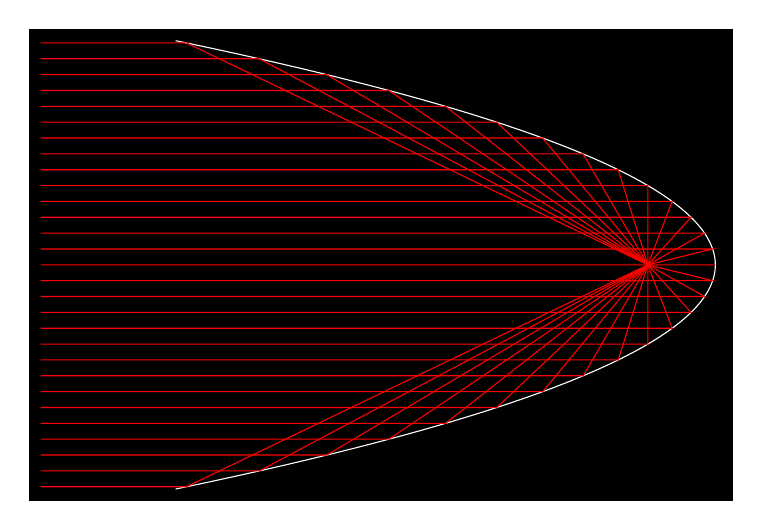
\begin{tikzpicture}[inverted,inverted]
  \begin{axis}[
    domain={-sqrt(2)}:{sqrt(2)},
    samples=100,
    axis y line=middle,
    axis x line=middle,
    axis line style={draw=none},
    tick style={draw=none},
    xticklabels=\empty,
    yticklabels=\empty,
    clip=false
    ]
    \addplot[smooth] (-x*x,x);
    \pgfplotsinvokeforeach{1.4,1.3,...,-1.4}{%
      \draw[red] (axis cs:-2.5,#1) -- (axis cs:{-#1*#1},#1) -- (axis cs:-0.25,0);
    }
  \end{axis}
\end{tikzpicture}
\end{document}
